The case study concerns a typical automatic management system for stock market investments, which consists of {\em n+1} participants:
the online stock market system and {\em n} investors, A$_i$, $i=1,\ldots, n$. Here, the resource will be the stocks of a company that the investors want to buy just in case the price falls below an established limit, which the investors fix previously by means of subscriptions, i.e., an investor subscribes to the resource (the stocks) with a certain guard (the value of the stocks he/she want to pay for it). The lifetime {\em lft} will be determined by the stock market system and the resource price will be fluctuating to simulate the rises/drops of the stock. Notice that we do not take into account the stock buy process since our aim is to model an investors' information system. Thus, the participants will be notified when their bids hold or the resource lifetime expires.  
Let us consider the choreography ${\it C=(O_{sys},O_1,\ldots,O_n)}$, where 
\mbox{${\it O_k=(PL_k,Var_k,A_k,A_{f{_k}},\mathcal{A}_{e{_k}})}$,~k=sys,~1,...,~n;}~\mbox{${\it Var_{sys}=}$} ${\it \{at,vEPR\}, Var_i=}$ \\ ${\it  \{v_i\},\ A_{f{_k}}= exit}$. Variable $v{EPR}$ serves to temporarily store the value of the resource property before being sent; $v_i$ is the variable used for the interaction among participants, and, finally, $at$ controls the period of time in which the auction is active. Note that the value {\em x} indicates the resource value at the beginning, {\em at0} is the time that the ``auction'' is active, and, finally, {\em $x_i$} is the value of the stocks that he/she wants to pay for. We assume that all variable values are initially $0$: 
%\vspace{-0.3cm}
\begin{flushleft}
\small{ 
${\it Asys=assign(x+1,vEPR);assign(at0,at);CreateResource(EPR,lft,x,empty);}$\\
\hspace{1.1cm}${\it  while(actualTime()<=at,Abid)}$\\
${\it Abid=getProp(EPR,vEPR);assign(vEPR+bid(),vEPR);setProp(EPR,vEPR);} $ \\ \hspace{1.1cm}${\it wait(1,2)}$\\
${\it A_i=wait(1,2);subscribe(O_i,EPR,EPR<x_i,Acond_i);} $ \\ \hspace{0.8cm}${\it pick((pl_i,buy,v_i,empty),empty,at0)}$\\
${\it Acond_i=getProp(EPR,vEPR);invoke(pl_i,buy,vEPR)}$\\
}
\end{flushleft}

Here, the function {\it bid} is used to increase/decrease the stocks value simulating the fluctuation of the stocks price.

\begin{figure}[h]
\fbox{
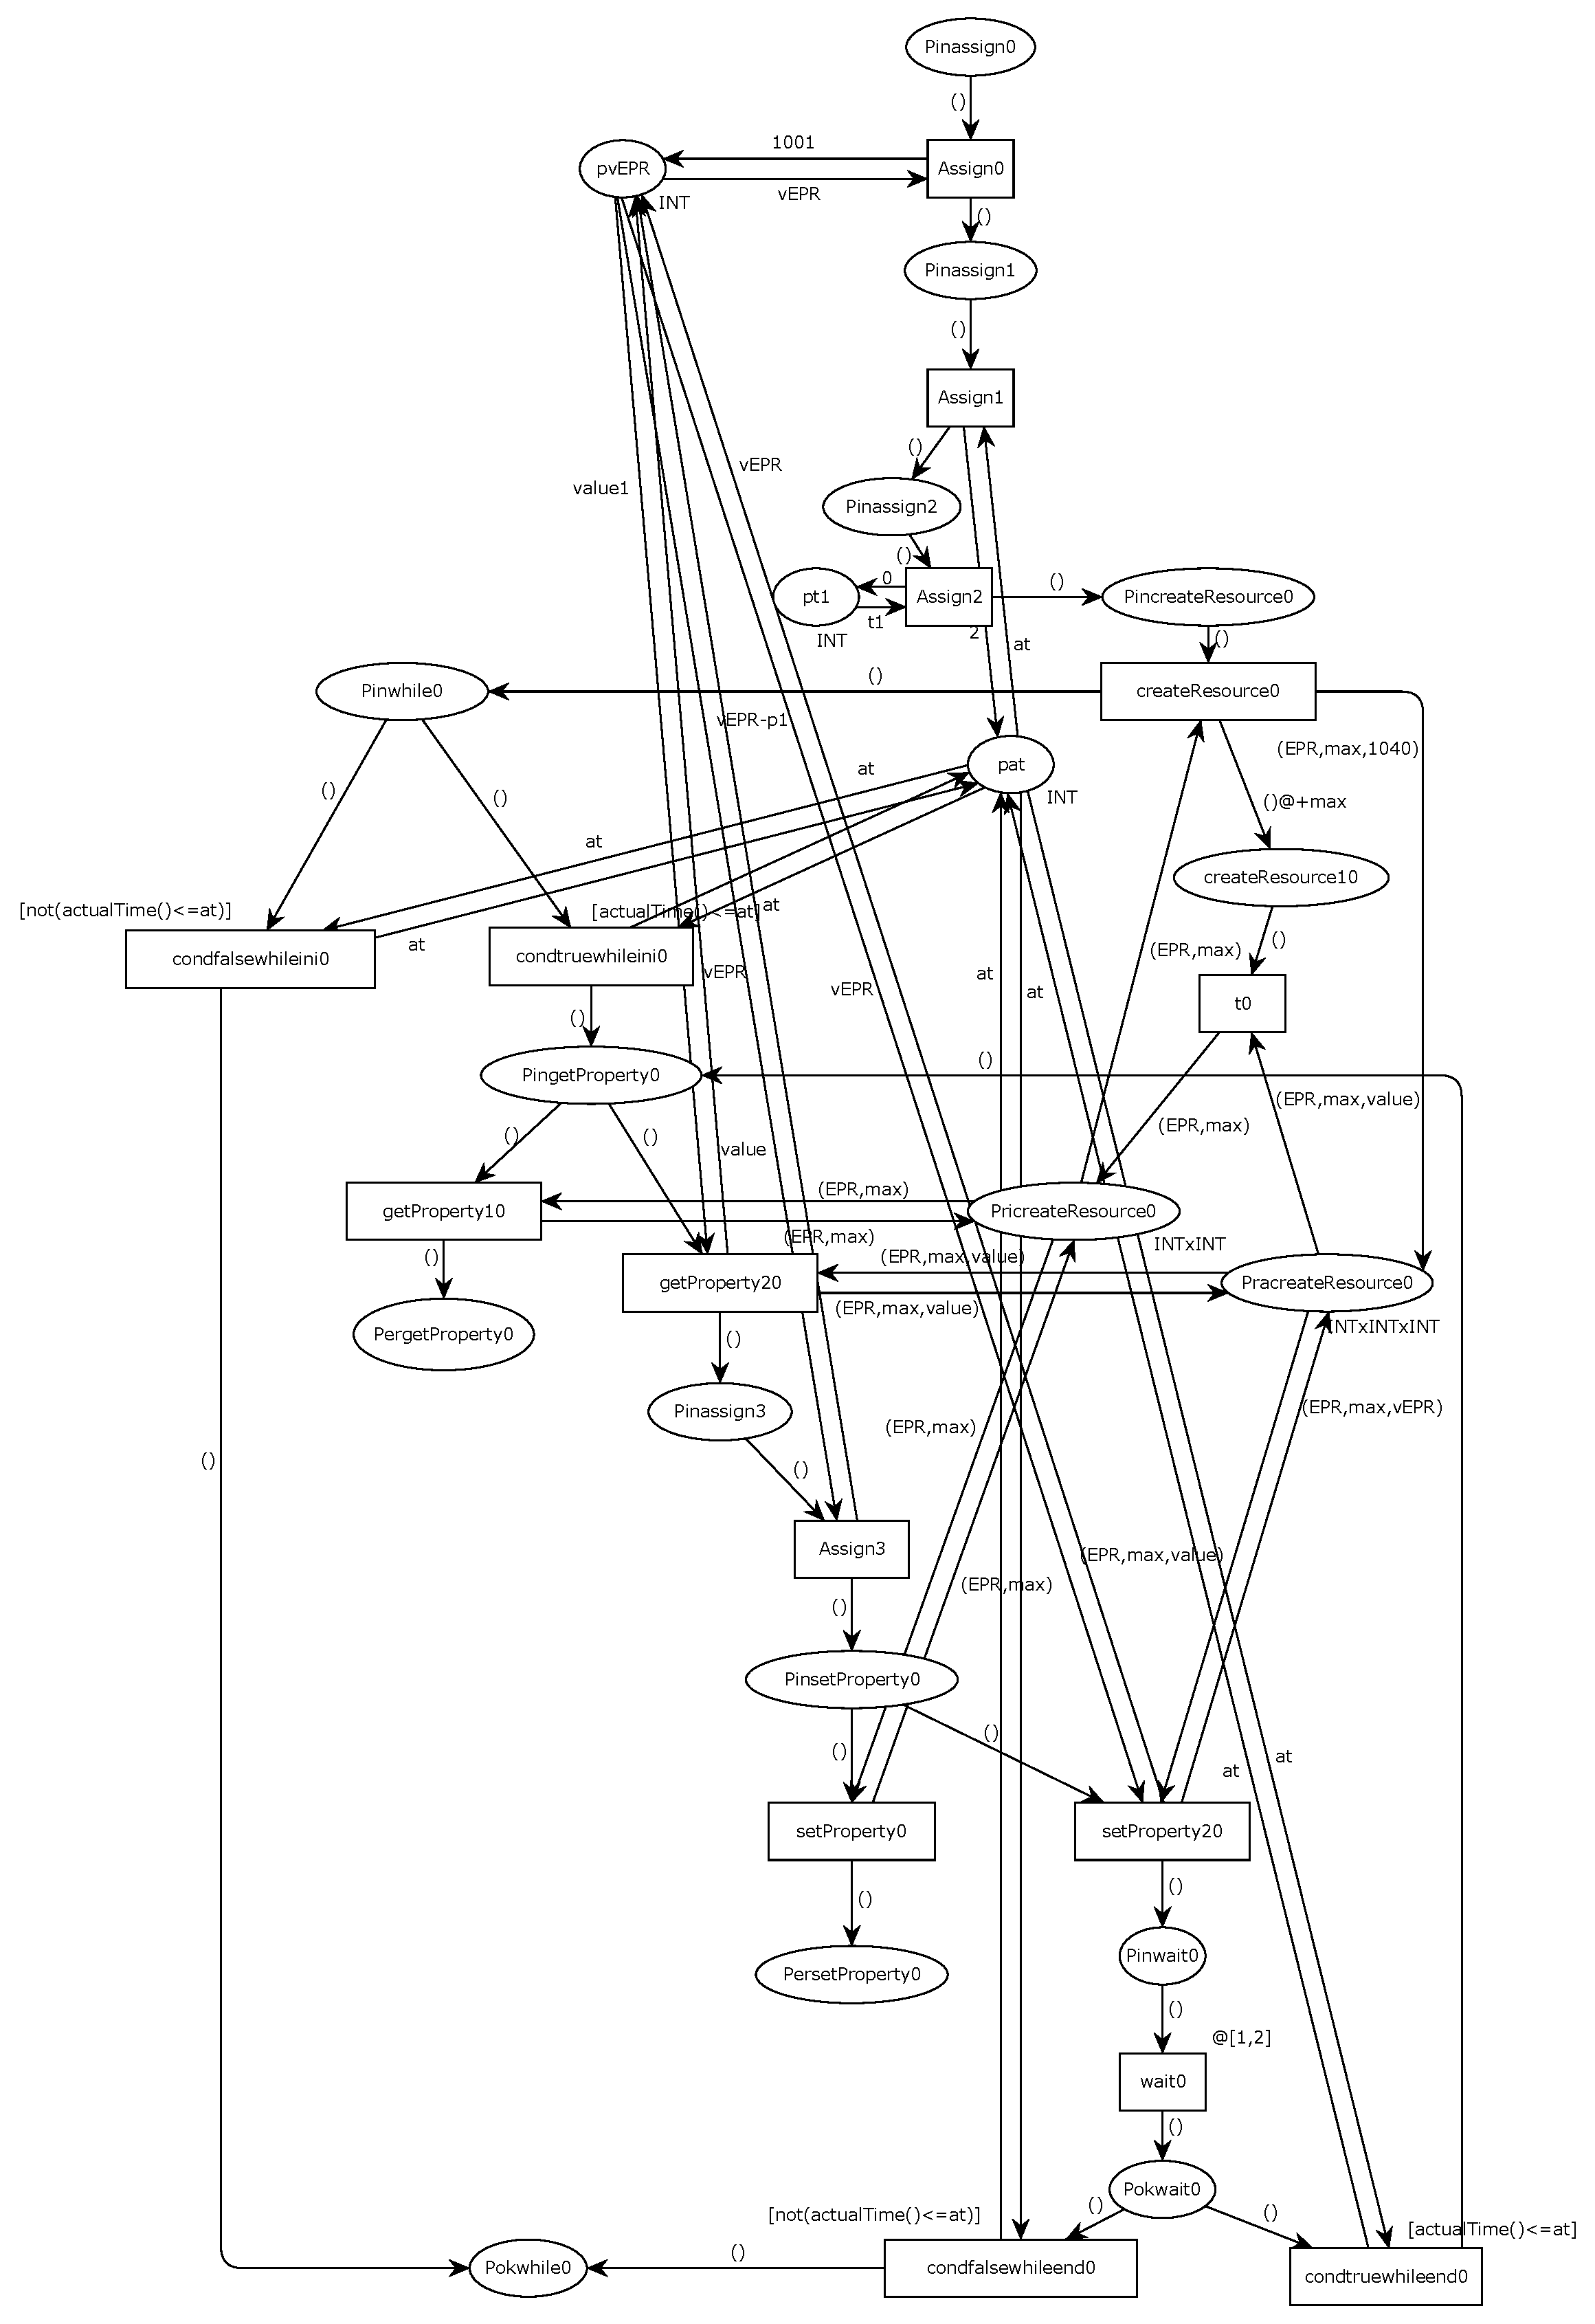
\includegraphics[width=\columnwidth, height=10cm]{Images/sistema.eps}}
\vspace{-0.4cm}
\caption{PTCPN of the online stock market.}\label{sistema}
\end{figure}
In Figs. \ref{sistema} and \ref{proceso}, the PTCPNs for one buyer and for the system are depicted.  These figures have been obtained automatically by using our tool \cite{Maria2012}. A beta version of our tool is available at \url{http://www.dsi.uclm.es/retics/bpelrf/}.
\begin{figure}[h]
\fbox{
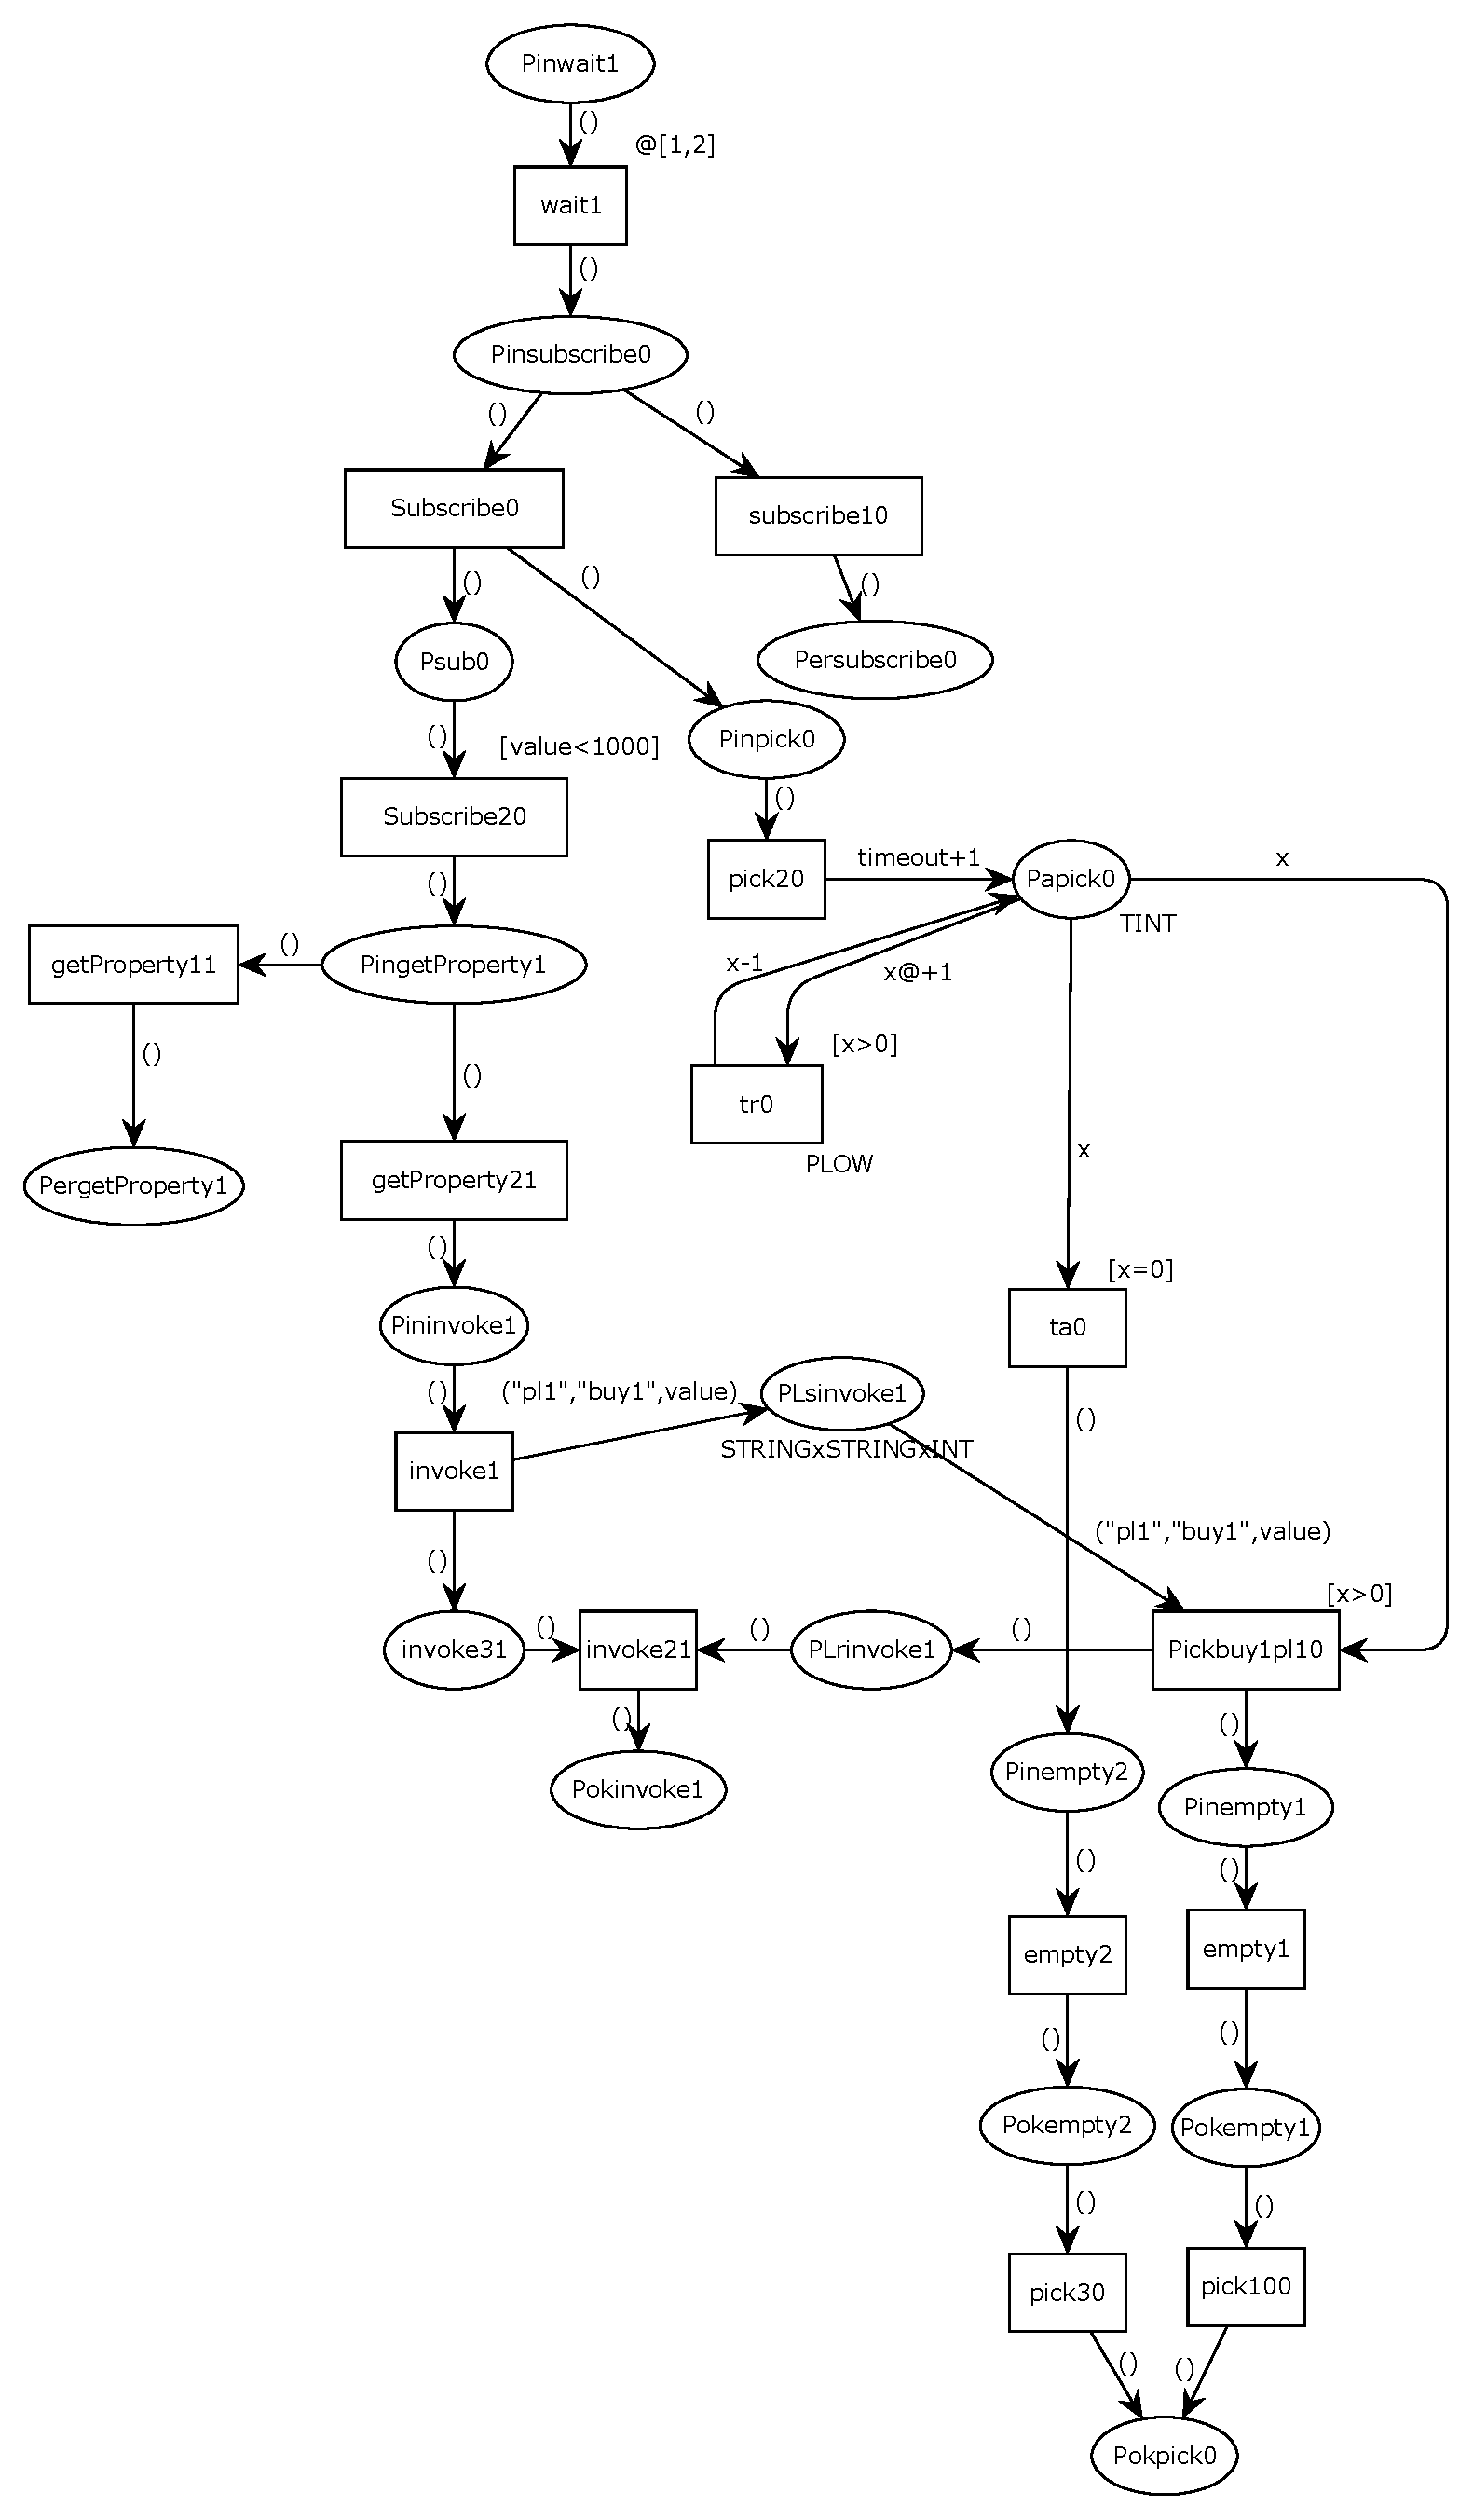
\includegraphics[width=\columnwidth, height=10cm]{Images/proceso.eps}}
\vspace{-0.4cm}
\caption{PTCPN of one buyer.}\label{proceso}
\end{figure}

